\section {EPICS Archiver Appliance}

\subsection {Introdução}

O EPICS Archiver Appliance, desenvolvido pelo instituto americano
\textit{National Accelerator Laboratory (SLAC)}, é capaz de monitorar e arquivar
um grande número de váriaveis, as chamadas \textit{PVs}, geradas por servidores
EPICS presentes na rede. O sistema fornence também opções de configuração de um
largo conjunto de parâmetros referentes ao armazenamento e monitoramento. Uma
\textit{appliance} é composta basicamente por quatro módulos distintos, sendo eles:

\begin{itemize}
  \renewcommand\labelitemi{--}
  \item \textit{Management}: provê as ferramentas necessárias para a gerência
  da \textit{appliance}. Permite, por exemplo, adicionar ou remover \textit{PVs}
  à lista de variáveis a serem arquivadas;
  \item \textit{Engine}: realiza a integração entre os módulos;
  \item \textit{Data Retrieval}: módulo responsável por recuperar os dados das
  \textit{PVs} arquivadas;
  \item \textit{ETL}: responsável por extrair os dados e tranformá-los a fim de
  que as aplicações possam processá-los posteriormente;
\end{itemize}

A figura \ref{fig:epics_archiver} esquematiza o modo de funcionamento do
\textit{EPICS Archiver Appliance}.

\FloatBarrier

\begin{figure}[h]
    
    \centering
    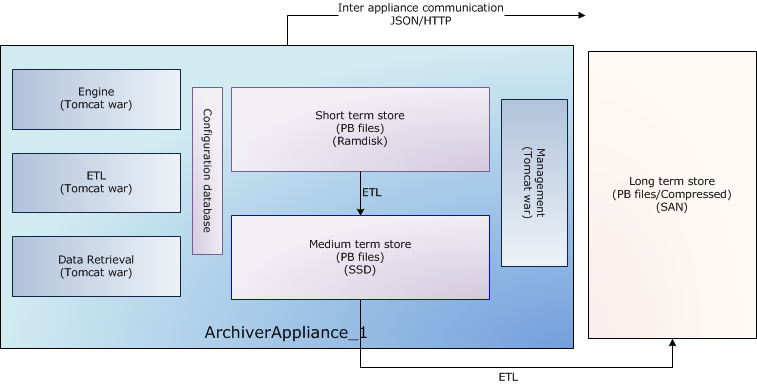
\includegraphics[scale=0.6]{image/applarch}
    \caption {Modo de funcionamento de uma \textit{appliance}}
    \label{fig:epics_archiver} 
\end{figure} 

\FloatBarrier

O instituto desenvolvedor da aplicação sugere que cada módulo seja lançada em
sua própria instância \textit{Tomcat}. Em adição, ele propõe a divisão da
unidade de armazenamento em 3 outras unidades, de acordo com a frequência que os
dados são salvos. Essas unidades são divididas \textit{short-term},
\textit{medium-term} e \textit{long-term storage}, cujas frequências de
armazenamento são, respectivamente, a cada hora, diária e anual. Essas
configurações podem ser modificadas através da modificação de arquivos
específicos, explicados nas próximas subseções.

\subsection {Instalação}

Esta subseção é dedicada às etapas necessárias para a instalação do EPICS
Archiver Appliance.

\subsubsection {Instalação das dependências}

A aplicação necessita, além da própria base de bibliotecas EPICS, da
instalação do \textit{java-jdk 8} e de servidores \textit{MySQL} e
\textit{Apache Tomcat}.

\begin {enumerate}[i.] 
  \item \textbf{Instalação do EPICS}: é necessário inicialmente fazer o
  \textit{download} e compilar as bibliotecas EPICS. Escolha um diretório de
  acordo com sua preferência (referenciado nesse documento por
  \texttt{\$EPICS\_DIR}) e execute os comandos abaixo. Alguns erros podem
  ocorrer na execução do comando \texttt{make}, resultantes da falta de algumas
  bibliotecas no sistema. Faça as respectivas instalações e repita o processo.
\begin{lstlisting}[language=bash, style=nonumbers]
$ cd $EPICS_DIR
$ wget http://www.aps.anl.gov/epics/download/base/baseR3.14.12.5.tar.gz
$ tar -xvzf baseR3.14.12.5.tar.gz
$ rm baseR3.14.12.5.tar.gz
$ cd base-3.14.12.5
$ make
\end{lstlisting}

Adicione as seguintes variáveis de ambiente ao arquivo \texttt{.bashrc} do seu
usuário (geralmente encontrado em \texttt{/home/user/}). Esse arquivo de
configuração é consultado toda vez que um usuário executa um novo
\textit{shell}.
\begin{lstlisting}[language=bash, style=nonumbers]
export PATH=$EPICS_DIR/base-3.14.12.5/bin/linux-x86_64:$PATH
export EPICS_BASE=$EPICS_DIR/base-3.14.12.5
export EPICS_HOST_ARCH=linux-x86_64
\end{lstlisting}	

Enfim, atualize a sessão com

\begin{lstlisting}[language=bash, style=nonumbers]
$ source /home/user/.bashrc
\end{lstlisting}	

Para testar a instalação, use o comando \texttt{caget} com
alguma variável disponível na sua rede.

\begin{lstlisting}[language=bash, style=nonumbers]
$ caget variavel
\end{lstlisting}

\item \textbf{Instalação do Java 8}: execute o comando abaixo para instalar o
\textit{Java Development Kit}.
\begin{lstlisting}[language=bash, style=nonumbers]
$ sudo apt-get install openjdk-8-jdk
\end{lstlisting}

O EPICS Archiver Appliance necessita de duas variáveis de ambiente referentes ao
\textit{Java}. Adicione-as no arquivo \textit{.bashrc}, após as variáveis de
ambiente EPICS.

\begin{lstlisting}[language=bash, style=nonumbers]
export JAVA_HOME="/usr/lib/jvm/java-8-openjdk-amd64"
export JRE_HOME="/usr/lib/jvm/java-8-openjdk-amd64/jre"
\end{lstlisting}

\item \textbf{Instalação do MySQL Server}: para instalar um servidor
\textit{MySQL}, basta executar o comando abaixo. Durante o processo de
instalação, será requisitada a senha para o usuário \textit{root} do servidor. 
\begin{lstlisting}[language=bash, style=nonumbers]
$ sudo apt-get install mysql-server
\end{lstlisting}

\item \textbf{Instalação do Apache Tomcat}: defina um diretório onde os arquivos
serão instalados e execute os comandos abaixo. Esse diretório será referenciado
pela variável de ambiente \texttt{\$TOMCAT\_DIR}.

\begin{lstlisting}[language=bash, style=nonumbers]
$ cd $TOMCAT_DIR
$ wget http://ftp.unicamp.br/pub/apache/tomcat/tomcat-8/v8.0.32/bin/apache-tomcat-8.0.32.tar.gz
$ tar -xvzf apache-tomcat-8.0.32.tar.gz
$ rm apache-tomcat-8.0.32.tar.gz
$ cd apache-tomcat-8.0.32/
\end{lstlisting}

Defina a variável de ambiente \texttt{\$CATALINA\_HOME}, responsável por
referenciar o diretório \textit{apache-tomcat-8.0.32/} recém criado. Adicione a
seguinte linha no arquivo \texttt{.bashrc} logo abaixo das variáveis de ambiente
adicionadas na instalação do \textit{Java}.

\begin{lstlisting}[language=bash, style=nonumbers]
export CATALINA_HOME = $TOMCAT_DIR/apache-tomcat-8.0.32
\end{lstlisting}

\end{enumerate} 

\subsubsection {Instalação do EPICS Archiver Appliance}

Tendo instalado todas as dependências, é necessário ainda configurar
alguns parâmetros e instalar os pacotes referentes ao arquivador. Para tal, crie
uma pasta onde serão instalados os pacotes. Esse diretório será referenciado por
\texttt{\$INSTALL\_DIR} neste documento.

\begin {enumerate}[i.] 
  \item Crie uma pasta e faça o \textit{download} dos pacotes do arquivador,
  segundo os comandos abaixo. 
\begin{lstlisting}[language=bash, style=nonumbers]
$ mkdir $INSTALL_DIR/epics-archiver-appliance/
$ cd $INSTALL_DIR/epics-archiver-appliance/
$ wget
https://github.com/slacmshankar/epicsarchiverap/releases/download/v0.0.1_SNAPSHOT_26-January-2016/archappl_v0.0.1_SNAPSHOT_26-January-2016T18-03-47.tar.gz
$ tar -xvzf archappl_v0.0.1_SNAPSHOT_26-January-2016T18-03-47.tar.gz
$ rm archappl_v0.0.1_SNAPSHOT_26-January-2016T18-03-47.tar.gz
\end{lstlisting}
	Nesta pasta estão os arquivos \textit{.war}  usados para lançar os módulos e
	alguns \textit{scripts} sugeridos pelo desenvolvedor para auxiliar na
	instalação.
  \item Crie uma pasta onde as instâncias \textit{Tomcat} de cada módulo serão
  armazenadas e crie o arquivo \textit{lnls\_appliances.xml}. Vamos chamar essa
  pasta de \texttt{epics-appliances/}. 
\begin{lstlisting}[language=bash, style=nonumbers]
$ mkdir $INSTALL_DIR/epics-appliances/
$ nano $INSTALL_DIR/epics-appliances/lnls_appliances.xml
\end{lstlisting}
Copie as seguintes linhas para esse arquivo: 
\begin{lstlisting}[language=bash, style=nonumbers]
<appliances>
   <appliance>
     <identity>lnls_epics_appliance</identity>
     <cluster_inetport>localhost:12000</cluster_inetport>
     <mgmt_url>http://localhost:11995/mgmt/bpl</mgmt_url>
     <engine_url>http://localhost:11996/engine/bpl</engine_url>
     <etl_url>http://localhost:11997/etl/bpl</etl_url>
     <retrieval_url>http://localhost:11998/retrieval/bpl</retrieval_url>
     <data_retrieval_url>http://localhost:11998/retrieval</data_retrieval_url>
   </appliance>
 </appliances>
\end{lstlisting} 
Esse arquivo especifica os endereços e portas de cada um dos quatro módulos, bem
como o nome da \textit{appliance} (\texttt{lnls\_epics\_appliance}). Os números
das portas foram escolhidos aleatoriamente, mas, por sugestão do desenvolver,
deve-se adotar uma sequência crescente a partir da porta do módulo
\texttt{mgmt}, que, no nosso caso, vale 11995.
\texttt{\(<\)data\_retrieval\_url\(>\)} é o endereço que deverá ser utilizado
a fim de enviar e obter requisões HTTP e JSON, conforme figura
\ref{fig:epics_archiver} e \texttt{\(<\)cluster\_inetport\(>\)} é a combinação
\texttt{TCPIP address:port} usado para a comunicação entre as
\textit{appliances}. Por fim, adicione as váriaveis de ambiente ao arquivo
\texttt{.bashrc}.

\begin{lstlisting}[language=bash, style=nonumbers]
export ARCHAPPL_APPLIANCES=$INSTALL_DIR/epics-appliances/lnls_appliances.xml
export ARCHAPPL_MYIDENTITY="lnls_epics_appliance"
\end{lstlisting}


O desenvolvedor sugere também trocar a porta padrão usada pelo \textit{Apache
Tomcat} pela porta usada pelo módulo \texttt{mgmt}, isto é, 11995, e comentar
as linhas sobre o uso do conector AJP. Para isso, siga a sequência abaixo.

\begin{lstlisting}[language=bash, style=nonumbers]
$ nano $CATALINA_HOME/conf/server.xml
### Edite a porta de forma a obter
[...]
<Connector port="11995" protocol="HTTP/1.1"
               connectionTimeout="20000"
               redirectPort="8443" />
[...]
### Comente o trecho
<!-- Define an AJP 1.3 Connector on port 8009 
    <Connector port="8009" protocol="AJP/1.3" redirectPort="8443" /> -->
\end{lstlisting}

Execute o \textit{script} disponibilizado pelo desenvolvedor para criar as 4
instâncias do \textit{Apache Tomcat}.

\begin{lstlisting}[language=bash, style=nonumbers]
$ source /home/user/.bashrc
$ cd $INSTALL_DIR/epics-archiver-appliance/install_scripts
$ ./deployMultipleTomcats.py $INSTALL_DIR/epics-appliances
\end{lstlisting}

Serão criadas 4 pastas dentro de \texttt{\$INSTALL\_DIR/epics-appliances}, uma
para cada módulo.

\item É possível também alteração as configurações de \textit{log}. O
desenvolvedor sugere que sejam executados os seguintes comandos:

\begin{lstlisting}[language=bash, style=nonumbers]
$ nano $CATALINA_HOME/lib/log4j.properties

### Arquivo log4j.properties
# Set root logger level and its only appender to A1.
log4j.rootLogger=ERROR, A1
log4j.logger.config.org.epics.archiverappliance=INFO
log4j.logger.org.apache.http=ERROR

# A1 is set to be a DailyRollingFileAppender
log4j.appender.A1=org.apache.log4j.DailyRollingFileAppender
log4j.appender.A1.File=arch.log
log4j.appender.A1.DatePattern='.'yyyy-MM-dd

# A1 uses PatternLayout.
log4j.appender.A1.layout=org.apache.log4j.PatternLayout
log4j.appender.A1.layout.ConversionPattern=%-4r [%t] %-5p %c %x - %m%n
\end{lstlisting}

\item O próximo passo é definir o arquivo \texttt{policies.py}. Esse arquivo
especifica as regras de armazenagem que serão utilizadas pelo arquivador. O
arquivo fornecido pelo desenvolver define, por exemplo, três modalidades de
armazenamento, que foram exemplificadas na subseção \textbf{Introdução}. É
possível ajustar neste arquivo parâmetros que alteram a taxa de armazenamento de
uma PV dependendo de sua taxa de aquisição, por exemplo. Para um primeiro
instante vamos usar esse arquivo fornecido, que está disponível na pasta
\texttt{WEB-INF/classes} dentro do arquivo \texttt{mgmt.war} em
\texttt{\$INSTALL\_DIR/epics-archiver-appliance/}. Copie-o para
\texttt{\$INSTALL\_DIR/epics-appliances/} e renomeie-o para
\texttt{lnls\_policies.xml}. Enfim, defina variáveis de ambiente usada por este
arquivo.

\begin{lstlisting}[language=bash, style=nonumbers]
export ARCHAPPL_POLICIES=$INSTALL_DIR/epics-appliances/lnls_policies.py
export ARCHAPPL_SHORT_TERM_FOLDER=$INSTALL_DIR/epics-storage
export ARCHAPPL_MEDIUM_TERM_FOLDER=$INSTALL_DIR/epics-storage
export ARCHAPPL_LONG_TERM_FOLDER=$INSTALL_DIR/epics-storage
\end{lstlisting}

As três últimas variáveis devem ser corretamente configuradas de acordo com a
disponibilidade de equipamentos, por exemplo. No nosso caso, um único diretório
é usado para os três tipos de armazenamento, sendo ele \texttt{epics-storage/}.

\item A próxima etapa é a criação de tabelas usadas pelo EPICS Archiver
Appliance. Vamos criar uma base chamada \texttt{lnls\_appliance\_database} e o
usuário \texttt{lnls\_user}, com todos os direitos de acesso a ela. No nosso
caso, a senha do usuário é \texttt{app1}. 

\begin{lstlisting}[language=bash, style=nonumbers]
$ mysql -u root -p
>> CREATE DATABASE lnls_appliance_database;
>> GRANT ALL ON lnls_appliance_database.* TO 'lnls_user'@localhost IDENTIFIED BY
'app1';
\end{lstlisting}

Acesse o servidor \textit{mysql} com esse usuário e execute o \textit{script}
de criação das tabelas disponibilizado pelo desenvolvedor:

\begin{lstlisting}[language=bash, style=nonumbers]
$ mysql -u lnls_user -p
>> USE lnls_appliance_database
>> source
$INSTALL_DIR/epics-archiver-appliance/install_scripts/archappl_mysql.sql
\end{lstlisting}

\item É necessário fazer o \textit{download} do conector \textit{MySQL} usado
pelo \textit{Apache Tomcat}.

\begin{lstlisting}[language=bash, style=nonumbers]
$ wget
https://dev.mysql.com/get/Downloads/Connector-J/mysql-connector-java-5.1.38.tar.gz
\end{lstlisting} 

Abra este arquivo e extraia \texttt{mysql-connector-java-5.1.38-bin.jar} para o
diretório \texttt{\$CATALINA\_HOME/lib/}. Abra o arquivo
\textit{conf/context.xml} e adicione dentro de \texttt{\(<\)Context\(>\)}:

\begin{lstlisting}[language=bash, style=nonumbers]
$ nano $CATALINA_HOME/conf/context.xml

<Context ...>
	<Resource   name="jdbc/archappl"
	      auth="Container"
	      type="javax.sql.DataSource"
	      factory="org.apache.tomcat.jdbc.pool.DataSourceFactory"
	      username="lnls_user"
	      password="app1" 
	      testWhileIdle="true"
	      testOnBorrow="true"
	      testOnReturn="false"
	      validationQuery="SELECT 1"
	      validationInterval="30000"
	      timeBetweenEvictionRunsMillis="30000"
	      maxActive="10" 
	      minIdle="2" 
	      maxWait="10000" 
	      initialSize="2"
	      removeAbandonedTimeout="60"
	      removeAbandoned="true"
	      logAbandoned="true"
	      minEvictableIdleTimeMillis="30000" 
	      jmxEnabled="true"
	      driverClassName="com.mysql.jdbc.Driver"
	      url="jdbc:mysql://localhost:3306/lnls_appliance_database"
	 />
</Context>
\end{lstlisting}

\item É necessário copiar e extrair todos os arquivos \textit{.war} presentes em
\texttt{epics-archiver-appliance/} para os respectivos diretórios
\texttt{webapps/}. Para tal, definimos:

\begin{lstlisting}[language=bash, style=nonumbers]
export DEPLOY_DIR=$INSTALL_DIR/epics-appliances
export WARSRC_DIR=$INSTALL_DIR/epics-archiver-appliance
\end{lstlisting}

E executamos:

\begin{lstlisting}[language=bash, style=nonumbers]
$ source /home/user/.bashrc

pushd ${DEPLOY_DIR}/mgmt/webapps && rm -rf mgmt*; cp ${WARSRC_DIR}/mgmt.war .; mkdir mgmt; cd mgmt; jar xf ../mgmt.war; popd; 
pushd ${DEPLOY_DIR}/engine/webapps && rm -rf engine*; cp ${WARSRC_DIR}/engine.war .; mkdir engine; cd engine; jar xf ../engine.war; popd; 
pushd ${DEPLOY_DIR}/etl/webapps && rm -rf etl*; cp ${WARSRC_DIR}/etl.war .; mkdir etl; cd etl; jar xf ../etl.war; popd; 
pushd ${DEPLOY_DIR}/retrieval/webapps && rm -rf retrieval*; cp ${WARSRC_DIR}/retrieval.war .; mkdir retrieval; cd retrieval; jar xf ../retrieval.war; popd;

\end{lstlisting}

\item Enfim, lance os 4 \textit{Tomcats}:

\begin{lstlisting}[language=bash, style=nonumbers]
$ source /home/user/.bashrc

$ export CATALINA_BASE=${DEPLOY_DIR}/mgmt;${CATALINA_HOME}/bin/catalina.sh start 
$ export CATALINA_BASE=${DEPLOY_DIR}/engine;${CATALINA_HOME}/bin/catalina.sh start 
$ export CATALINA_BASE=${DEPLOY_DIR}/etl;${CATALINA_HOME}/bin/catalina.sh start 
$ export CATALINA_BASE=${DEPLOY_DIR}/retrieval; ${CATALINA_HOME}/bin/catalina.sh start

\end{lstlisting}

\item O arquivador é acessado através da URL 

\begin{lstlisting}[language=bash, style=nonumbers]
http://localhost:11995/mgmt/ui/index.html
\end{lstlisting}

\end{enumerate} 
